1;95;0c

\documentclass[letterpaper,aps,prl,superscriptaddress,floatfix,twocolumn]{revtex4}

\usepackage{graphicx}
%\usepackage[scientific-notation=true]{siunitx}
\usepackage{amsmath}
\usepackage{amssymb}
\usepackage{booktabs}
\usepackage{rotating}
\usepackage[]{units}
%\usepackage{caption}
\graphicspath{ {./Analysis-Primer/Primer_Images/} }

\begin{document}

\title{MARATHON Pass 2 Analysis Primer}

\author{Jason Bane}
\author{Tyler Hague}
\author{Tyler Kutz}
\author{Hanjie Liu}
\author{Mike Nycz}
\author{Tong Su}

\author{Evan McClellan}
%\affiliation{Thomas Jefferson National Accelerator Facility}


\date{\today}

\begin{abstract}
\end{abstract}

\maketitle

\section{I. Overview}

\section{II. Replay}
 (Tyler Hague)

\section{III. Calibrations}

 \subsection{i. E/p}
 (Mike Nycz)

 \subsection{ii. VDC}

 \subsection{iii. BPM}
\subsection{BPM PreBeam Check}




 \subsection{iv. Raster}
 (Tyler Hague)
 The Hall A Raster system was calibrated using a combination of the BPMs, Carbon Hole target, and Carbon Single Foil target. The goal of a successful calibration is to convert the ADC readout of the raster current into a beam position. To do this, a central position of the beam and a conversion factor from ADC readout to beam position deviation from the center.

In Hall A, we have two sets of raster coils working in tandem for the 12 GeV era. These rasters are synced to ensure that they work together, rather than against each other. With this knowledge, the Hall A Analyzer is set up so that the signals from a single raster set are used to determine the beam position. In our case, the analysis code is set up to use the upstream raster coils.

To determine the conversion from ADC to position for the horizontal direction in the hall reference frame (referred to as 'x' from here), we use the Carbon Single Foil Target. When the raster is properly calibrated in the x direction, there should be no correlation between the beam x position and the reconstructed z position of events. To do this, the z position of physics events are sliced in bins of beam x and then fit with a gaussian. The peak position of the each gaussian is then plotted versus the corresponding x position and fit with a line. Doing this method twice with two different preliminary (incorrect) calibrations allows for the slopes to be interpolated to the calibration that would yield no slope (no correlation).

This same procedure can be used with a momentum feature (e.g. the Hydrogen Elastic Peak) to calibrate the vertical direction in the hall reference frame ('y'). However, in the MARATHON kinematics there is no such momentum feature available. As an alternative, the carbon hole is fit to determine the calibration with the knowledge that it is 2mm in diameter. The fit is done using a radial sigmoid function to account for smearing that occurs during reconstruction. A sigmoid is a continuous function that approaches a step function as a "hardness" factor is approaches infinity.

The function used is:
\begin{equation}
\frac{[0]}{1+e^{-[5]*\left(\left([1]*\left([2]-x\right)\right)^{2}+\left([3]*\left([4]-y\right)\right)^{2}-1\right)}}+[6]
\end{equation}

In this function:
\begin{tabular}{l|l}
	\multicolumn{2}{l}{Variable Definitions}
	\hline
	$[0]$ & \\
	$[1]$ & \\
	$[2]$ & \\
	$[3]$ & \\
	$[4]$ & \\
	$[5]$ & \\
	$[6]$ & \\
\end{tabular}

Using the sigmoid fit, we found that the edge determined by the fit (the halfway point on the curve) was incorrect. This was discovered by looking at the correlation between the reconstructed x position of the beam and the reconstructed z of the events. However, we can guess that the "true" edge lies at approximately the same point on the curve in both x and y. Using the known conversion for x from the Carbon Single Foil Target, we can determine the position on the curve of the edge and then slide that along the contour of the sigmoid to determine the edge in y.


 \subsection{v. BCM}
\subsection{Unser and Beam Current Monitors Calibration}
In order to accurately calibrate the BCM's, first the unser must be calibrated. The unser is used as an absolute reference to which the BCM's are calibrated to. The procedure to calibrate the unser involves sending a constant and known currents through a thin wire inside of the unser. A series of currents with, over a range between 2.5 - 100 $\mu$A,during 90 second intervals, as can be seen in figure (??). which shows the frequency response of the unser for the various currents. A linear fit of sent current vs the unser response, determines an overall gain factor for the unser. The gain of the unser of calibrated 4 times during MARATHON before each BCM calibration was preformed, in order to check the unser's stability. Figure(??) shows the unser was stable during the entirety of the MARATHON run. 

\begin{table}[ht]
\caption{Unser Calibration Results}
%\centering
\begin{center}
\begin{tabular}{l| c| c| c| r}
Date & 03-05 & 03-28 & 4-03 & 04-06  \\
\hline
Unser Gain & 2.526e-4 & 2.524e-4 & 2.529e-4 & 2.527e-4\\
\end{tabular}
\end{center}
\end{table}

Having calibrated the unser, we can then calibrate the BCMs in a similar manner to the calibration of the unser but replacing the current from a wire with current from the electron beam. For the BCM calibrations during MARATHON and all Tritium experiments, the range in current was between 3 - 22.5 $\mu$A. Again, the procedure intervals of 90 seconds (i.e 90 seconds of continuous current to the Hall followed by 90 seconds with no beam). 
The Calibration procedure requires making cuts in the frequency response of the unser and BCM receiver and integrating the total amount of frequency to determine the average frequency of the receiver during the given time interval. An example of the cuts made is shown in figure 3

The unser frequency during the calibration can be related to the delivered current using the gain factor determined from the unser calibration. 
\begin{equation}
I_{unser} = gain * f_{unser}
\end{equation}

By then plotting $I_{unser} vs freq_{BCM}$ and fitting with a linear function, the gain and offset (which are proportional the slope and intercept of the fit respectively) of each BCM receiver can be determined. The gain 



%unser
\begin{figure}[H]
\begin{center}
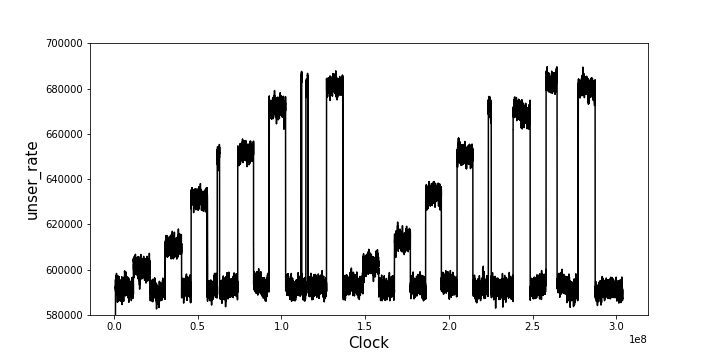
\includegraphics[angle=0, scale =0.65]{Unser_freq.png}
\end{center}
\caption{BCM Calibration : unser}
\end{figure}
%dnew
\begin{figure}[H]
\begin{center}
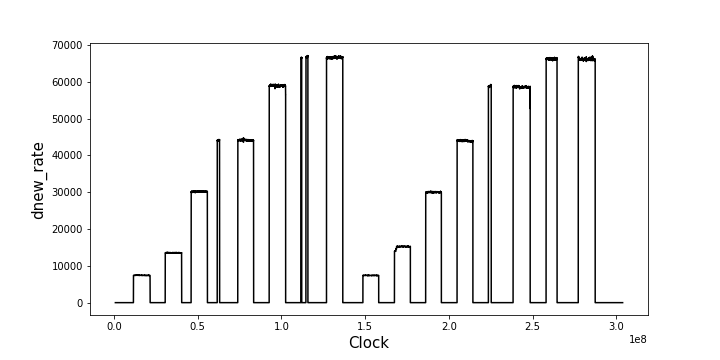
\includegraphics[angle=0, scale =0.65]{Dnew_freq.png}
\end{center}
\caption{BCM Calibration : dnew}
\end{figure}


\begin{figure}[H]
\begin{center}
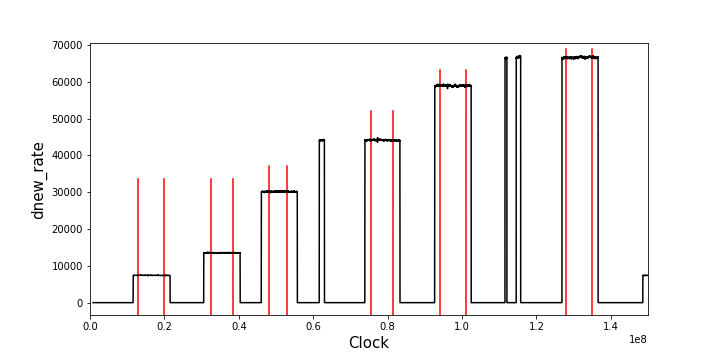
\includegraphics[angle=0, scale =0.65]{Dnew_freq_cuts.png}
\end{center}
\caption{Frequency cuts}
\end{figure}

Table(??) shows the result of the 3 BCM calibrations for the dnew digital BCM receiver.
\begin{table}[ht]
\caption{BCM Calibration Results}
%\centering
\begin{center}
\begin{tabular}{l| c| c| r}
   & 03-05 & 03-28 & 4-03 \\
\hline
dnew Gain & 3.3358e-4 & 3.3351e-4 & 3.3372e-4\\
\hline
dnew offset & -0.097  &   0.003   & 0.132         \\
\end{tabular}
\end{center}
\end{table}


 
 \subsection{vi. Optics}

\section{IV. Corrections}

 \subsection{i. PID}
 (Tong Su)
 


%opening

\section{The Traditional PID Efficiency Study and MARATHON PID Difficulty}
Each arm of the HRS has two particle identification: Gas Cherenkov and Lead Glass calorimeter. Compare to the other hadrons, both of these two detectors are much more sensitive to the electrons and their PID performance is independent. In the analysis, we use these two features by applying a cut on the calibrated Cherenkov ADC sum signals and calorimeter energy (or E/P) signals to distinguish the electrons and not only that these two features can also provide us a way to check the efficiency of these two PID cuts. The tradition way \cite{pid_eff} to check the PID cut efficiency is to apply a tight cut on one of the PID detectors to select a pure electron(pion) sample and check their performance on the other detectors . The electron(pion) efficiency for the checking cut can caculated by:
\begin{equation}\label{pid_eq1}
\epsilon_{pid-cut}=\dfrac{N'}{N_{sample}}
\end{equation}  
Where the $N_{sample}$ is number of events in the selecting sample and the $N'$ is the number of the events can pass the checking cut in the selecting sample.

For MARATHON experiment, we notice that except the traditional background signals which are inseneitive for both PID detectors(X2), there is another kind “particle” (X1) can introduce a large signal in the gas Cherenkov detector which behaves very similar to electron in the Cherenkov but can barely fire the calorimeter which is clearly different than what we expected electron performance in it(Shown in the Fig \ref{pid1}).
\begin{figure}[htbp]

\subfigure[kin1]{
\begin{minipage}[t]{1\linewidth}
\centering
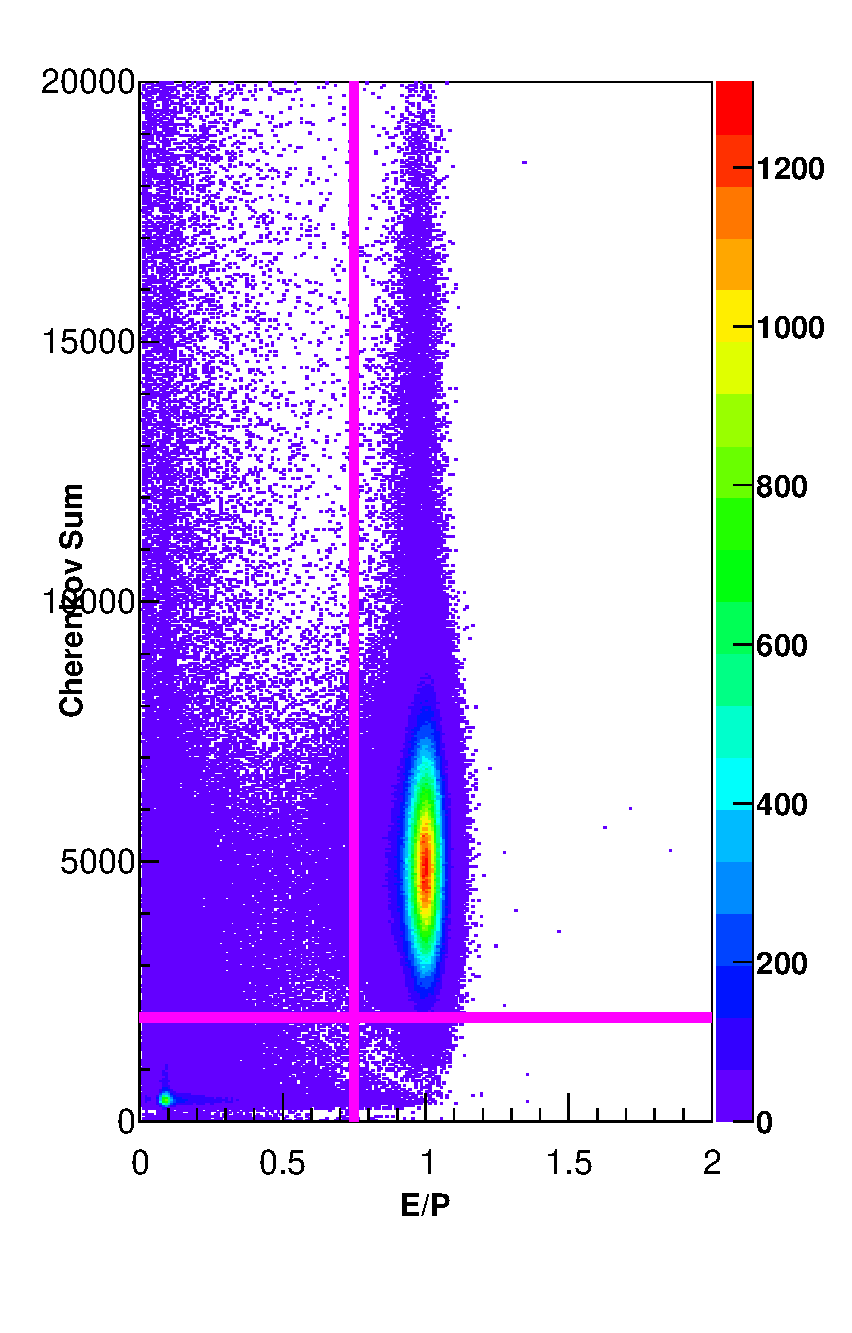
\includegraphics[width=2in]{./pid_plot/pid1.eps}
\end{minipage}
}\\
\centering
\subfigure[kin15]{
\begin{minipage}[t]{1\linewidth}
\centering
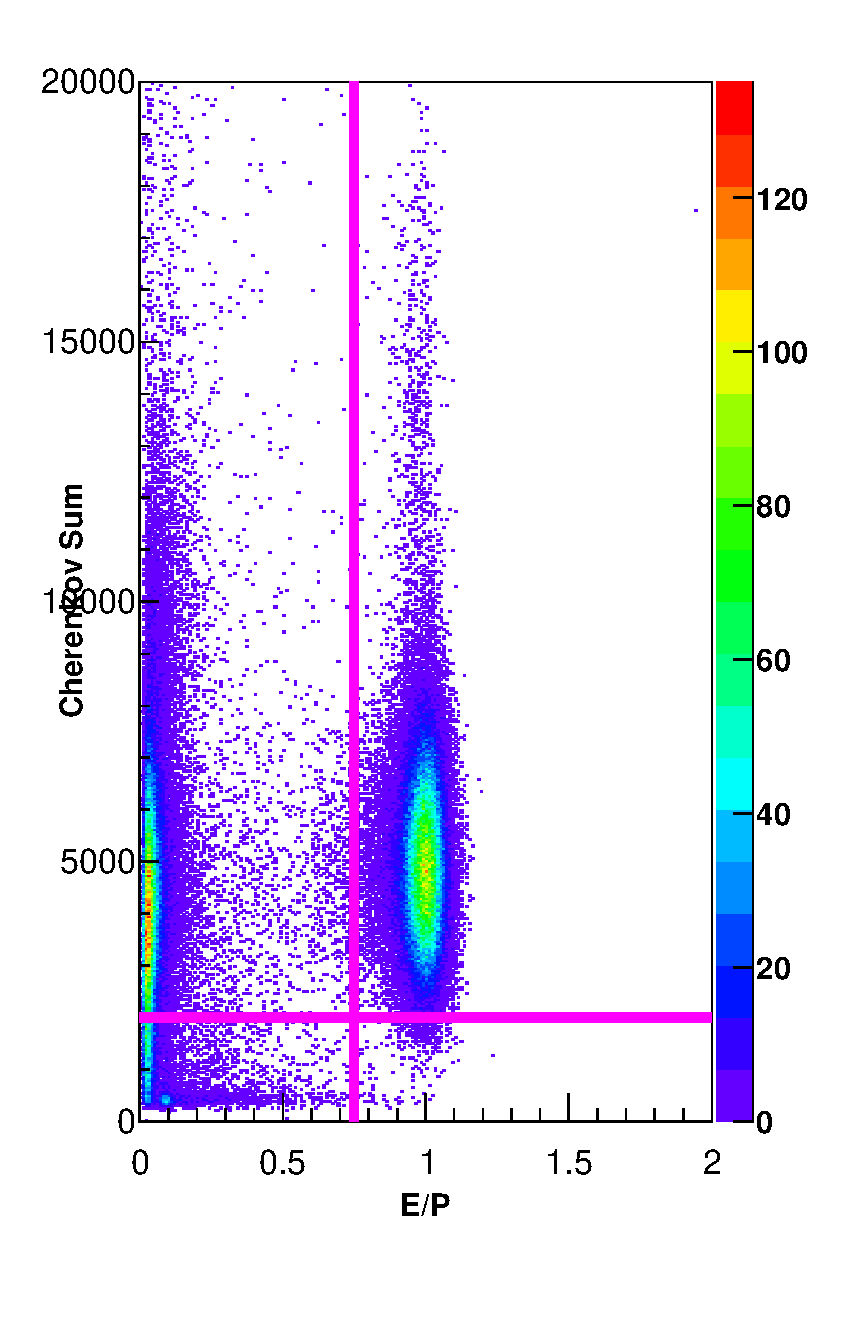
\includegraphics[width=2in]{./pid_plot/pid2.eps}
\end{minipage}
}
\centering
\caption{The 2 PID detector performance for $^{3}H$ at two differnet kinematics setting. General acceptance cut, T2 trigger cut, single track cut and a postive beta cut applied. The two magenta lines indicate the two cut postions for the Cherenkov(horizontal,2000) and E/P(vertical 0.7).  As we can see, different kinematics the ratio of X1 and X2 are different}
\label{pid1}
\end{figure}
The possible explanations for these suspicious signals including 1) for 11 GeV scattering, the high energy neutral particles hitting the back of the HRS dipole and getting into the acceptance and 2) the muon from $\pi^{0}$ decay can have chance to get into the acceptance and have chance to introduce big signal in the Cherenkov. To identify what exactly these signals are still need some work but because of the existence of these signals, there will be a challenge to use the traditional way to check the PID cut efficiency since the as shown in the Table \ref{sample1}, almost no clean sample can be selected out. 
\begin{table}[!ht]
\large
\centering
 \caption{Possibility to cut a pure sample from individual PID detectors}\label{tab:tablenotes}
\begin{threeparttable}
\begin{tabular}[t]{|c|c|c|}\hline
  Experimental Settings & Cherenkov & Calorimeter  \\ \hline        
  electron          &   $\times$ & $\surd$ \\ \hline
  X1                 &  $\times$  & difficult \\  \hline
 X2                  & $\times$  &   difficult\\  \hline  

 \end{tabular}
\begin{tablenotes}
\centering
        \item[1]  $ \times $ means "No", $ \surd $ means "Yes"
 \end{tablenotes}
\end{threeparttable}
\label{sample1} 
 \end{table}
\section{A compromised solution for the PID efficiency check}
Despite that more than one kind of the signals can fire gas Cherenkov and three peaks can be introduced in the calorimeter, if only electrons signals are taken care, we can treat the two calorimeter insensitive signals as a whole non-electron signals and define the four efficiency  in the Table \ref{eff1} 

\begin{table}[!ht]
\large
\centering
 \caption{efficiency defination for the 2 PID detectors}\label{tab:tablenotes}
\begin{tabular}[t]{|c|c|}\hline
   
  $P_{a}^{x}$          &   non-electrons efficiency for Cherenkov \\ \hline
  $P_{a}^{e}$                  &  electrons efficiency for Cherenkov \\  \hline
  $P_{b}^{x}$                 & non-electrons efficiency for Calrimator \\  \hline  
  $P_{b}^{e}$          &    electron efficiency for Calrimator \\  \hline

 \end{tabular}
 \label{eff1}
 \end{table}

After treating all the non-electrons signals as a whole, a clean sample of electron (or non-electron) can be selected form the calorimeter(Table \ref{sample2} and Fig \ref{sample3})
\begin{table}[!ht]
\large
\centering
 \caption{Possibility to cut a pure sample from individual PID detectors}\label{tab:tablenotes}
\begin{threeparttable}
\begin{tabular}[t]{|c|c|c|}\hline
  Experimental Settings & Cherenkov & Calorimeter  \\ \hline        
  electron          &   $\times$ & $\surd$ \\ \hline
  non-electron                &  $\times$  & $\surd$ \\  \hline
 \end{tabular}
\begin{tablenotes}
\centering
        \item[1]  $ \times $ means cannot, $ \surd $ means can
 \end{tablenotes}
\end{threeparttable}
\label{sample2}
 \end{table}
 
\begin{figure}
 	\begin{center}
 		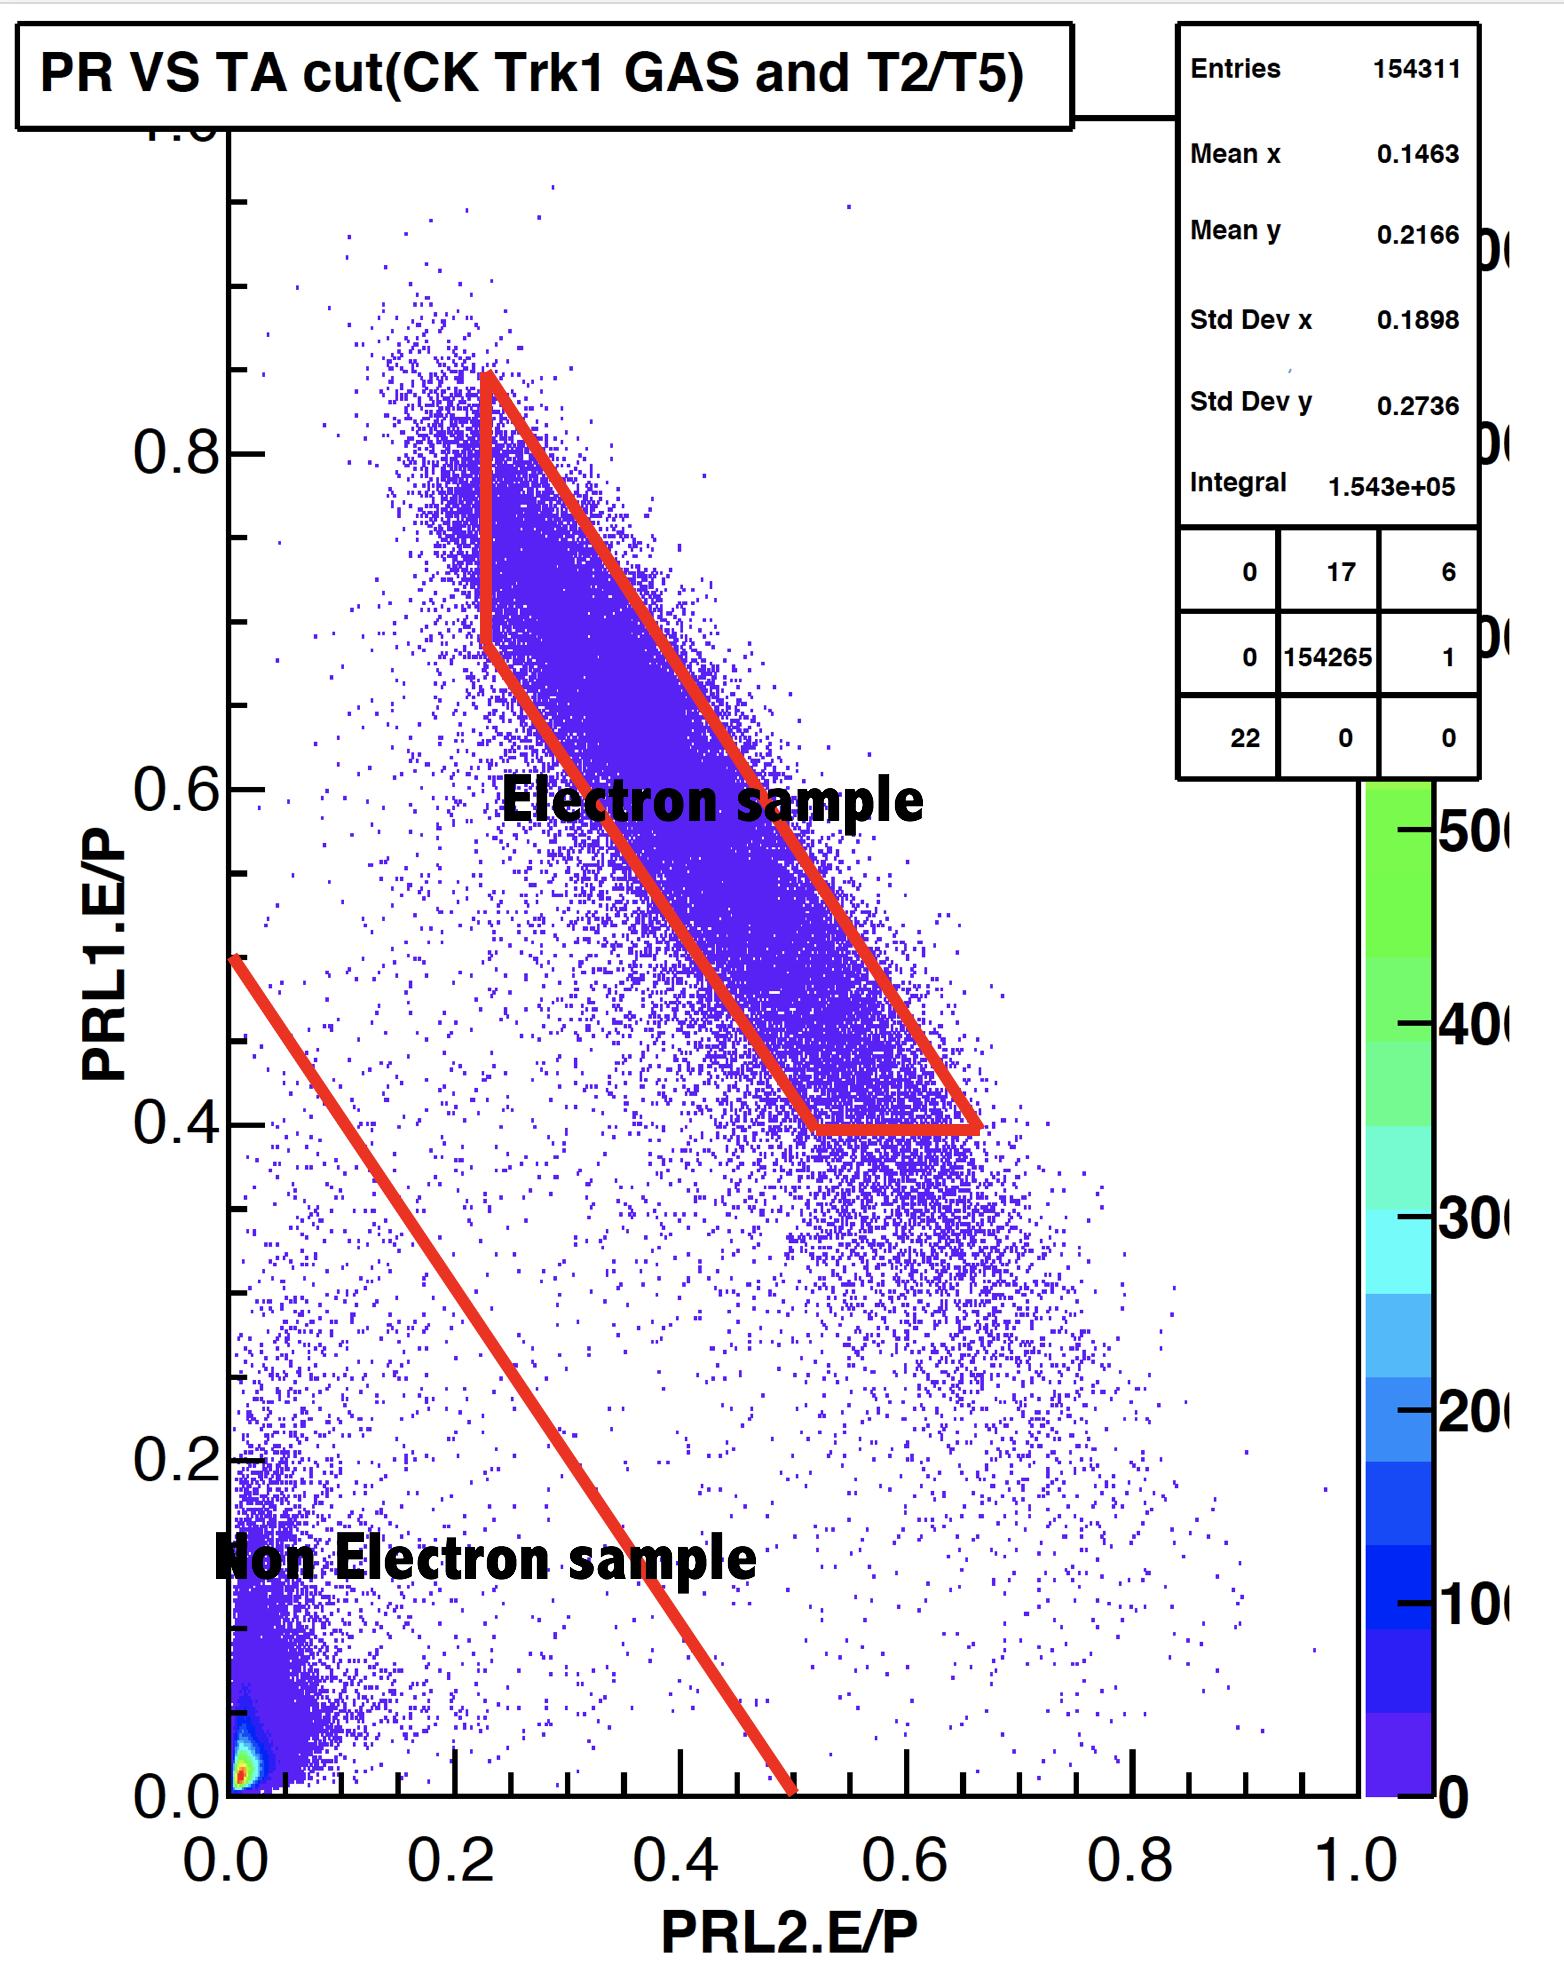
\includegraphics[width=0.4\textwidth] {./pid_plot/PID3.png}
 		\caption{electron and non-electron selecting from the calorimeter } \label{sample3}
 	\end{center}
\end{figure}   
 
 
then according the traditional way to check PID efficiency, the $P_{a}^{x}$ and $P_{a}^{e}$ can be calculable base on the Eq \ref{pid_eq1}. Since Cherenkov should behave stable for electron so the $P_{a}^{e}$ should be very close to 1 and its fluctuation should be very small by different kinematic settings. $P_{a}^{x}$ by contrast, is an effective efficiency for two different kinds signals which can be varied by different kinematic settings because of the different rations of X1 and X2 . Utilizing the independence of the two detectors and the following four functions

\begin{equation}  
\left\{  
             \begin{array}{lr}  
             N_{e}+N_{x}=N_{0} \\  
             P_{a}^{e} N_{e}+ P_{a}^{x} N_{x}=N_{1} \\    
             P_{b}^{e} N_{e}+ P_{b}^{x} N_{x}=N_{2} \\     
             P_{a}^{e} P_{b}^{e} N_{e}+ P_{a}^{x} P_{b}^{x} N_{x}=N_{3}\\  
             \end{array}  
\right.  
\label{PID_eq2}
\end{equation}  

The $P_{b}^{e}$,$P_{b}^{x}$,$N_{x}$,$N_{e}$ can be solved. Where the $N_{0}$ is the event number with the following general cut
\begin{equation}  \label{pid_eq3}
\left\{  
             \begin{array}{lr}  
             No \quad of \quad Track ==1 \\  
             -60\quad mrad< \theta_{tg} <60 \quad mrad \\    
             -30\quad mrad<\varphi_{tg} <30\quad  mrad  \\     
             -0.04<dp<0.04\\
             \beta>0  \\
             T2 \quad trigger\quad only
             \end{array}  
\right.  
\end{equation}  
$N_{1}(N_{2})$is the event number with just  additional Cherenkov (E/P) cut  and $N_{3}$ is the event number with two pid detector cut. $N_{x}(N_{e}) $ is the number of non-electrons(electrons) totally in our data after the previous cut. 

The following four plots(Fig \ref{PPID3} and Fig \ref{PPID4}) shows the four efficiencies defined previous for the two PID detectors, and as we can see three of them ($P_{b}^{e}$,$P_{b}^{x}$,$P_{a}^{e}$) are behaved stable for different kinematics and the $P_{a}^{x}$ varies as what we expected.
\begin{figure}[htpb]

\subfigure[electron effciency for Cherenkov]{
\begin{minipage}[t]{1\linewidth}

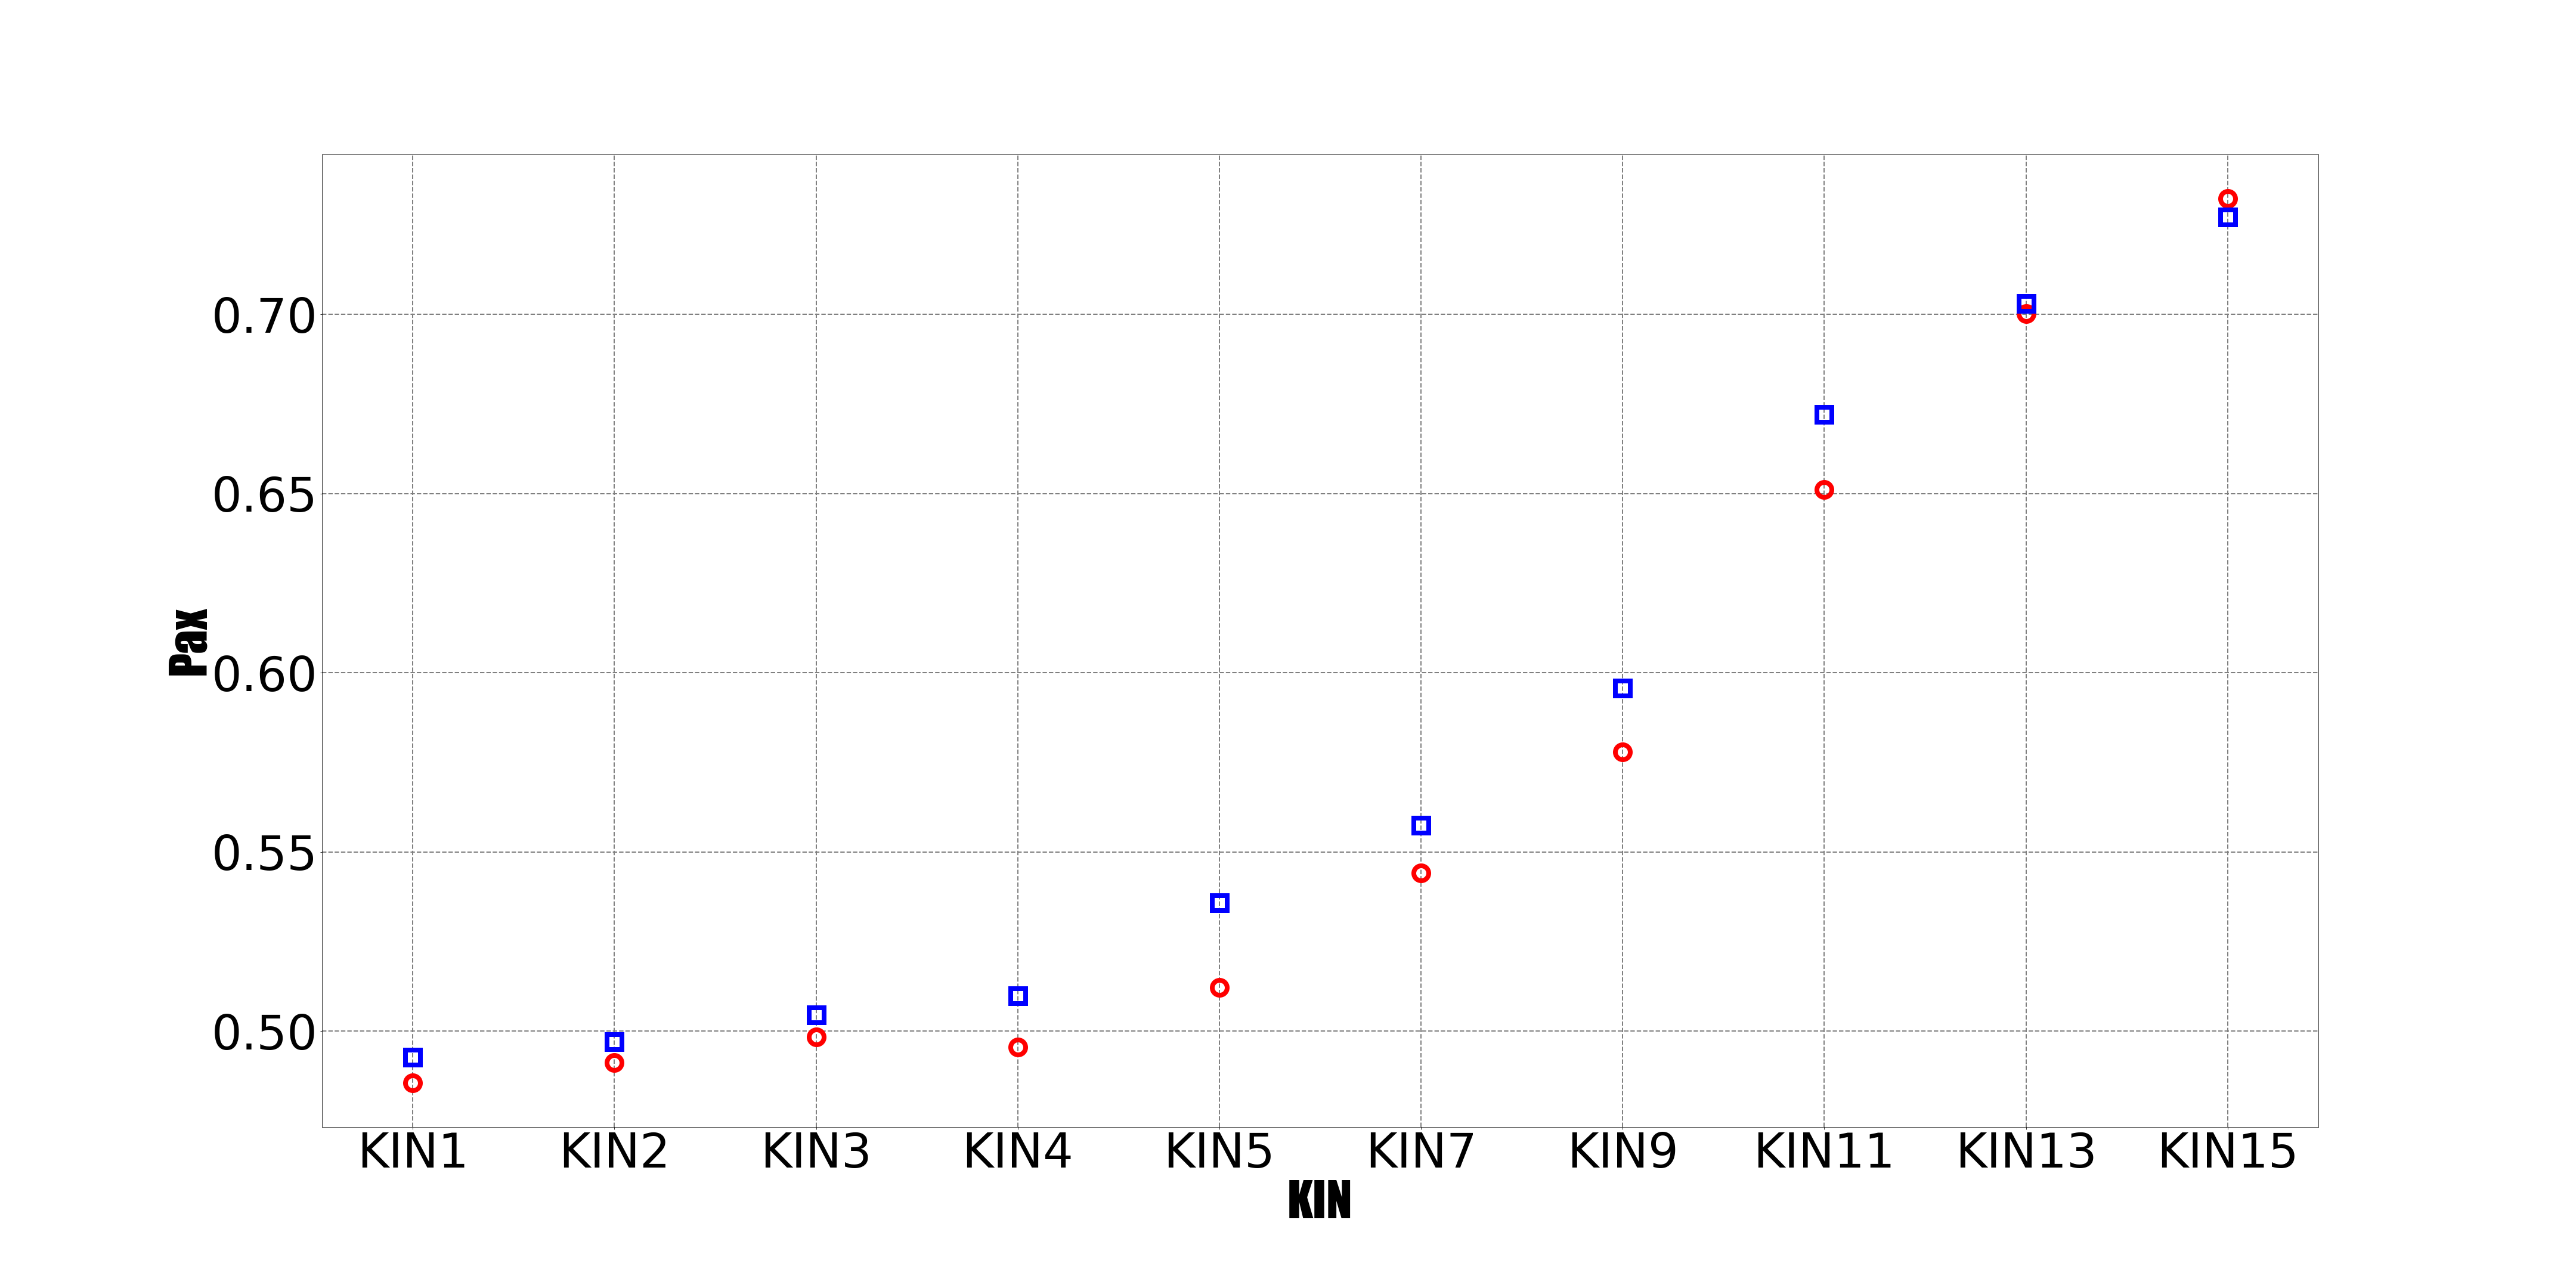
\includegraphics[width=3in]{./pid_plot/PIDD1.png}
\end{minipage}
}
\subfigure[non-electron effciency for Cherenkov]{
\begin{minipage}[t]{1\linewidth}

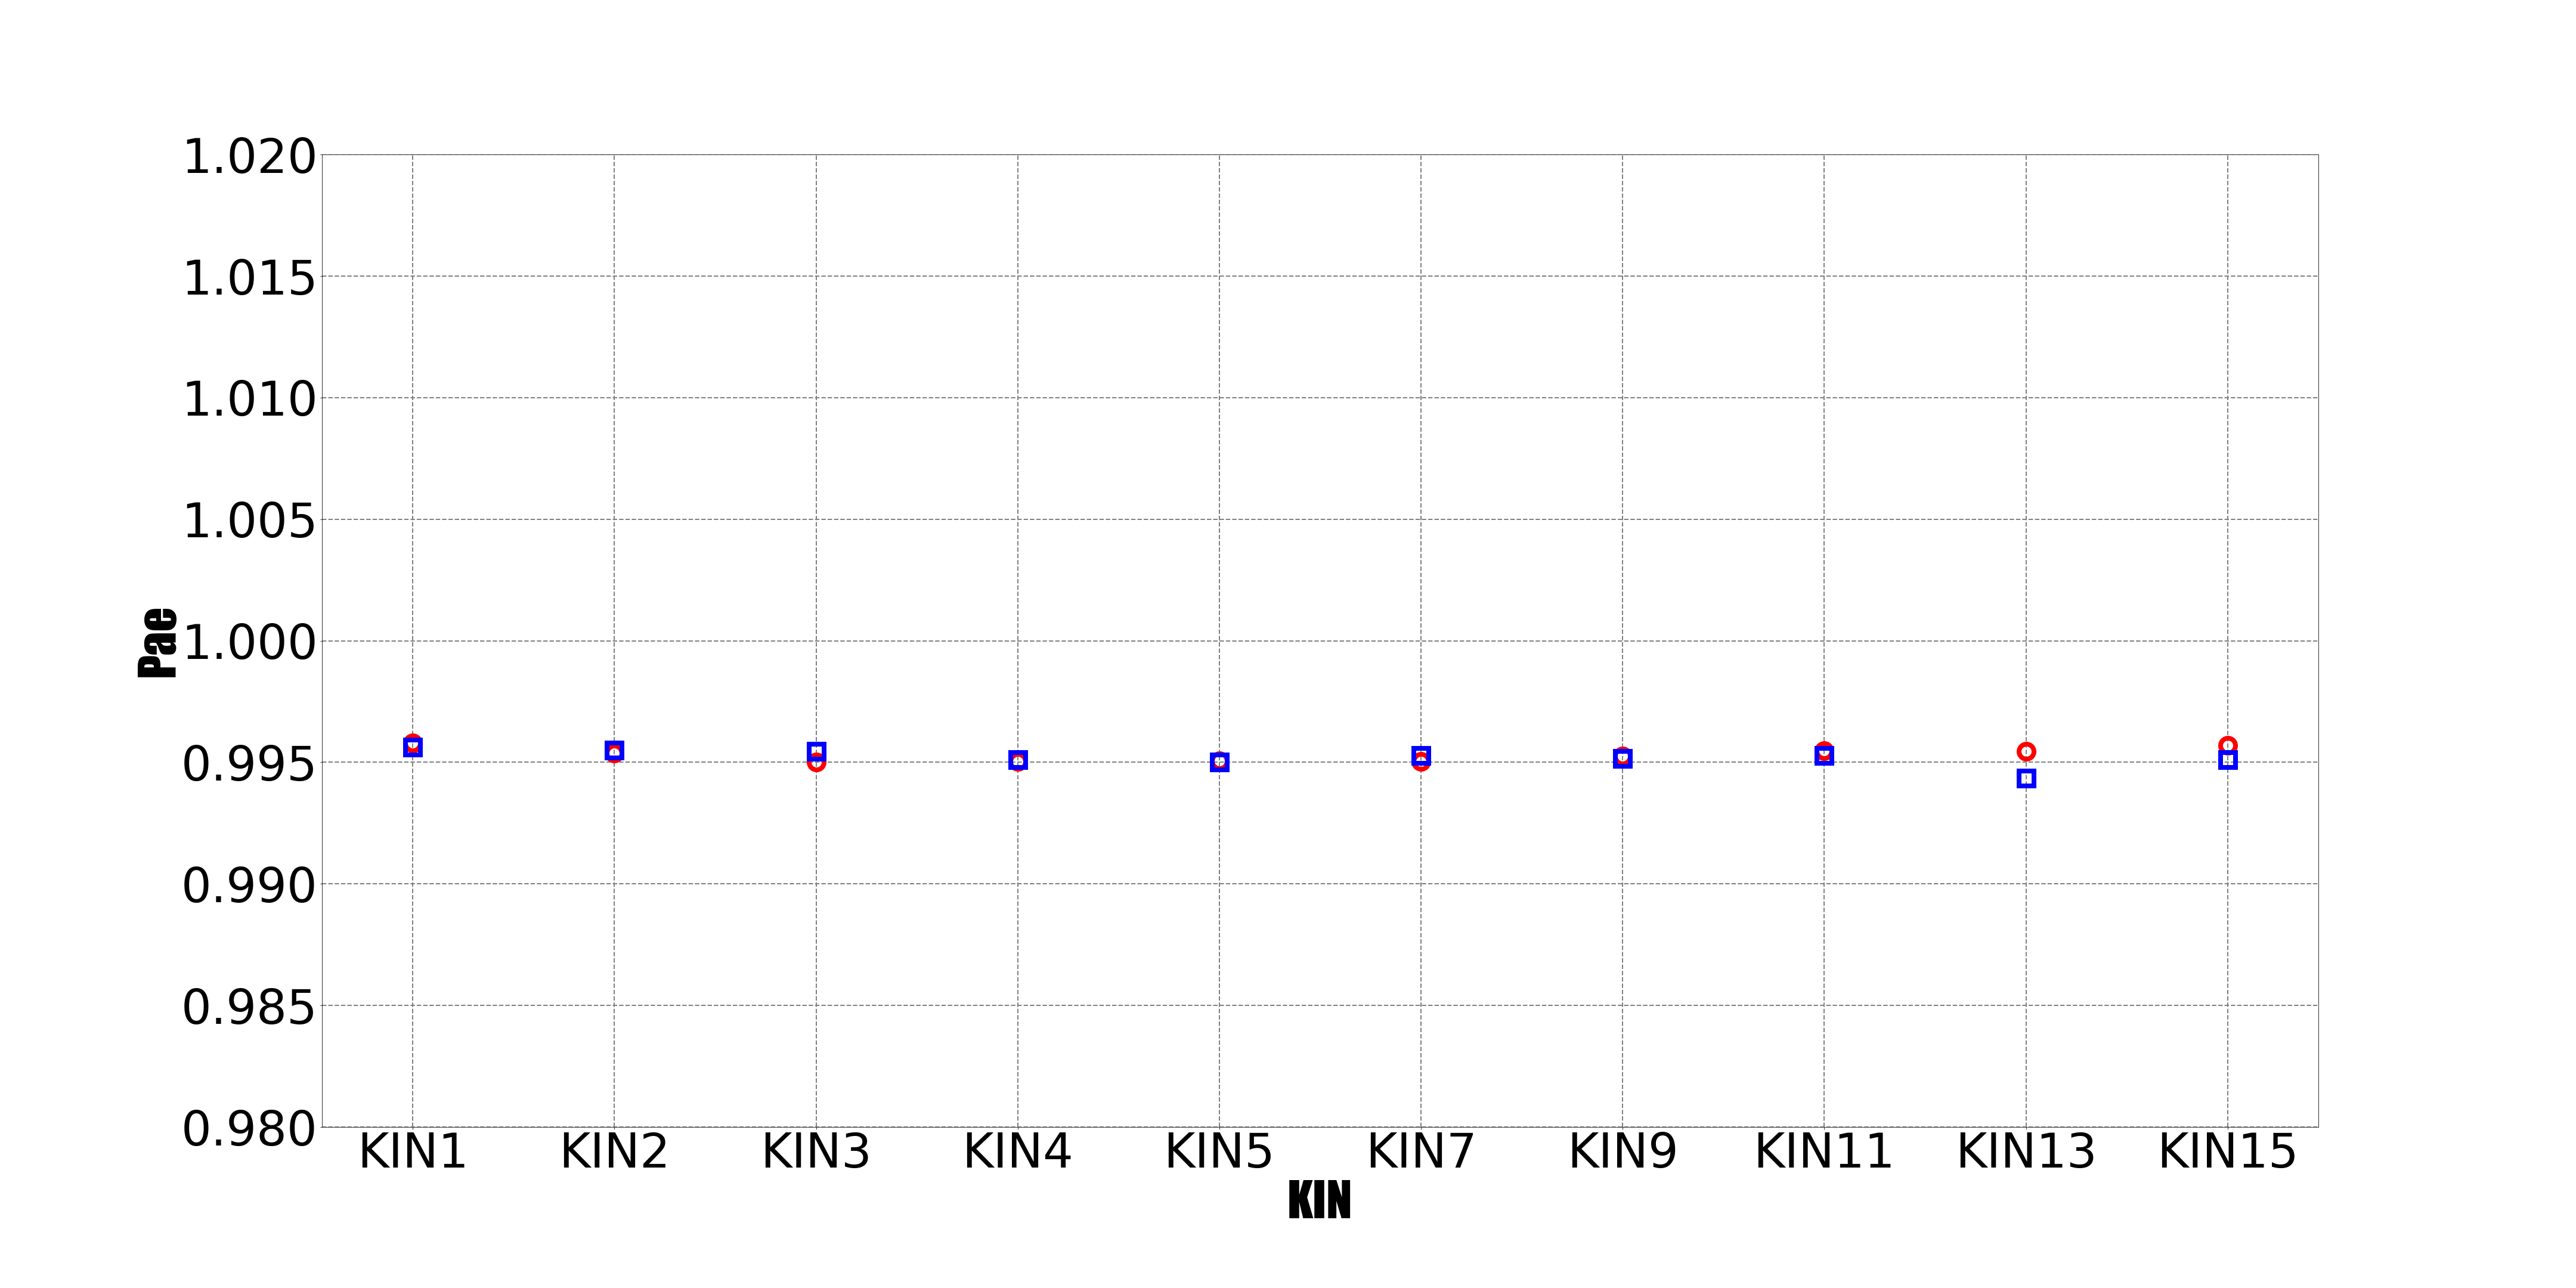
\includegraphics[width=3in]{./pid_plot/PIDD2.png}
\end{minipage}
}

\caption{The two PID efficiency for Chenerkov with different kinematic settings (Blue: He3 and Red: H3)  }  \label{PPID3}
\end{figure}

\begin{figure}[htpb] 
\subfigure[electron effciency for calorimeter ]{
\begin{minipage}[t]{1\linewidth}

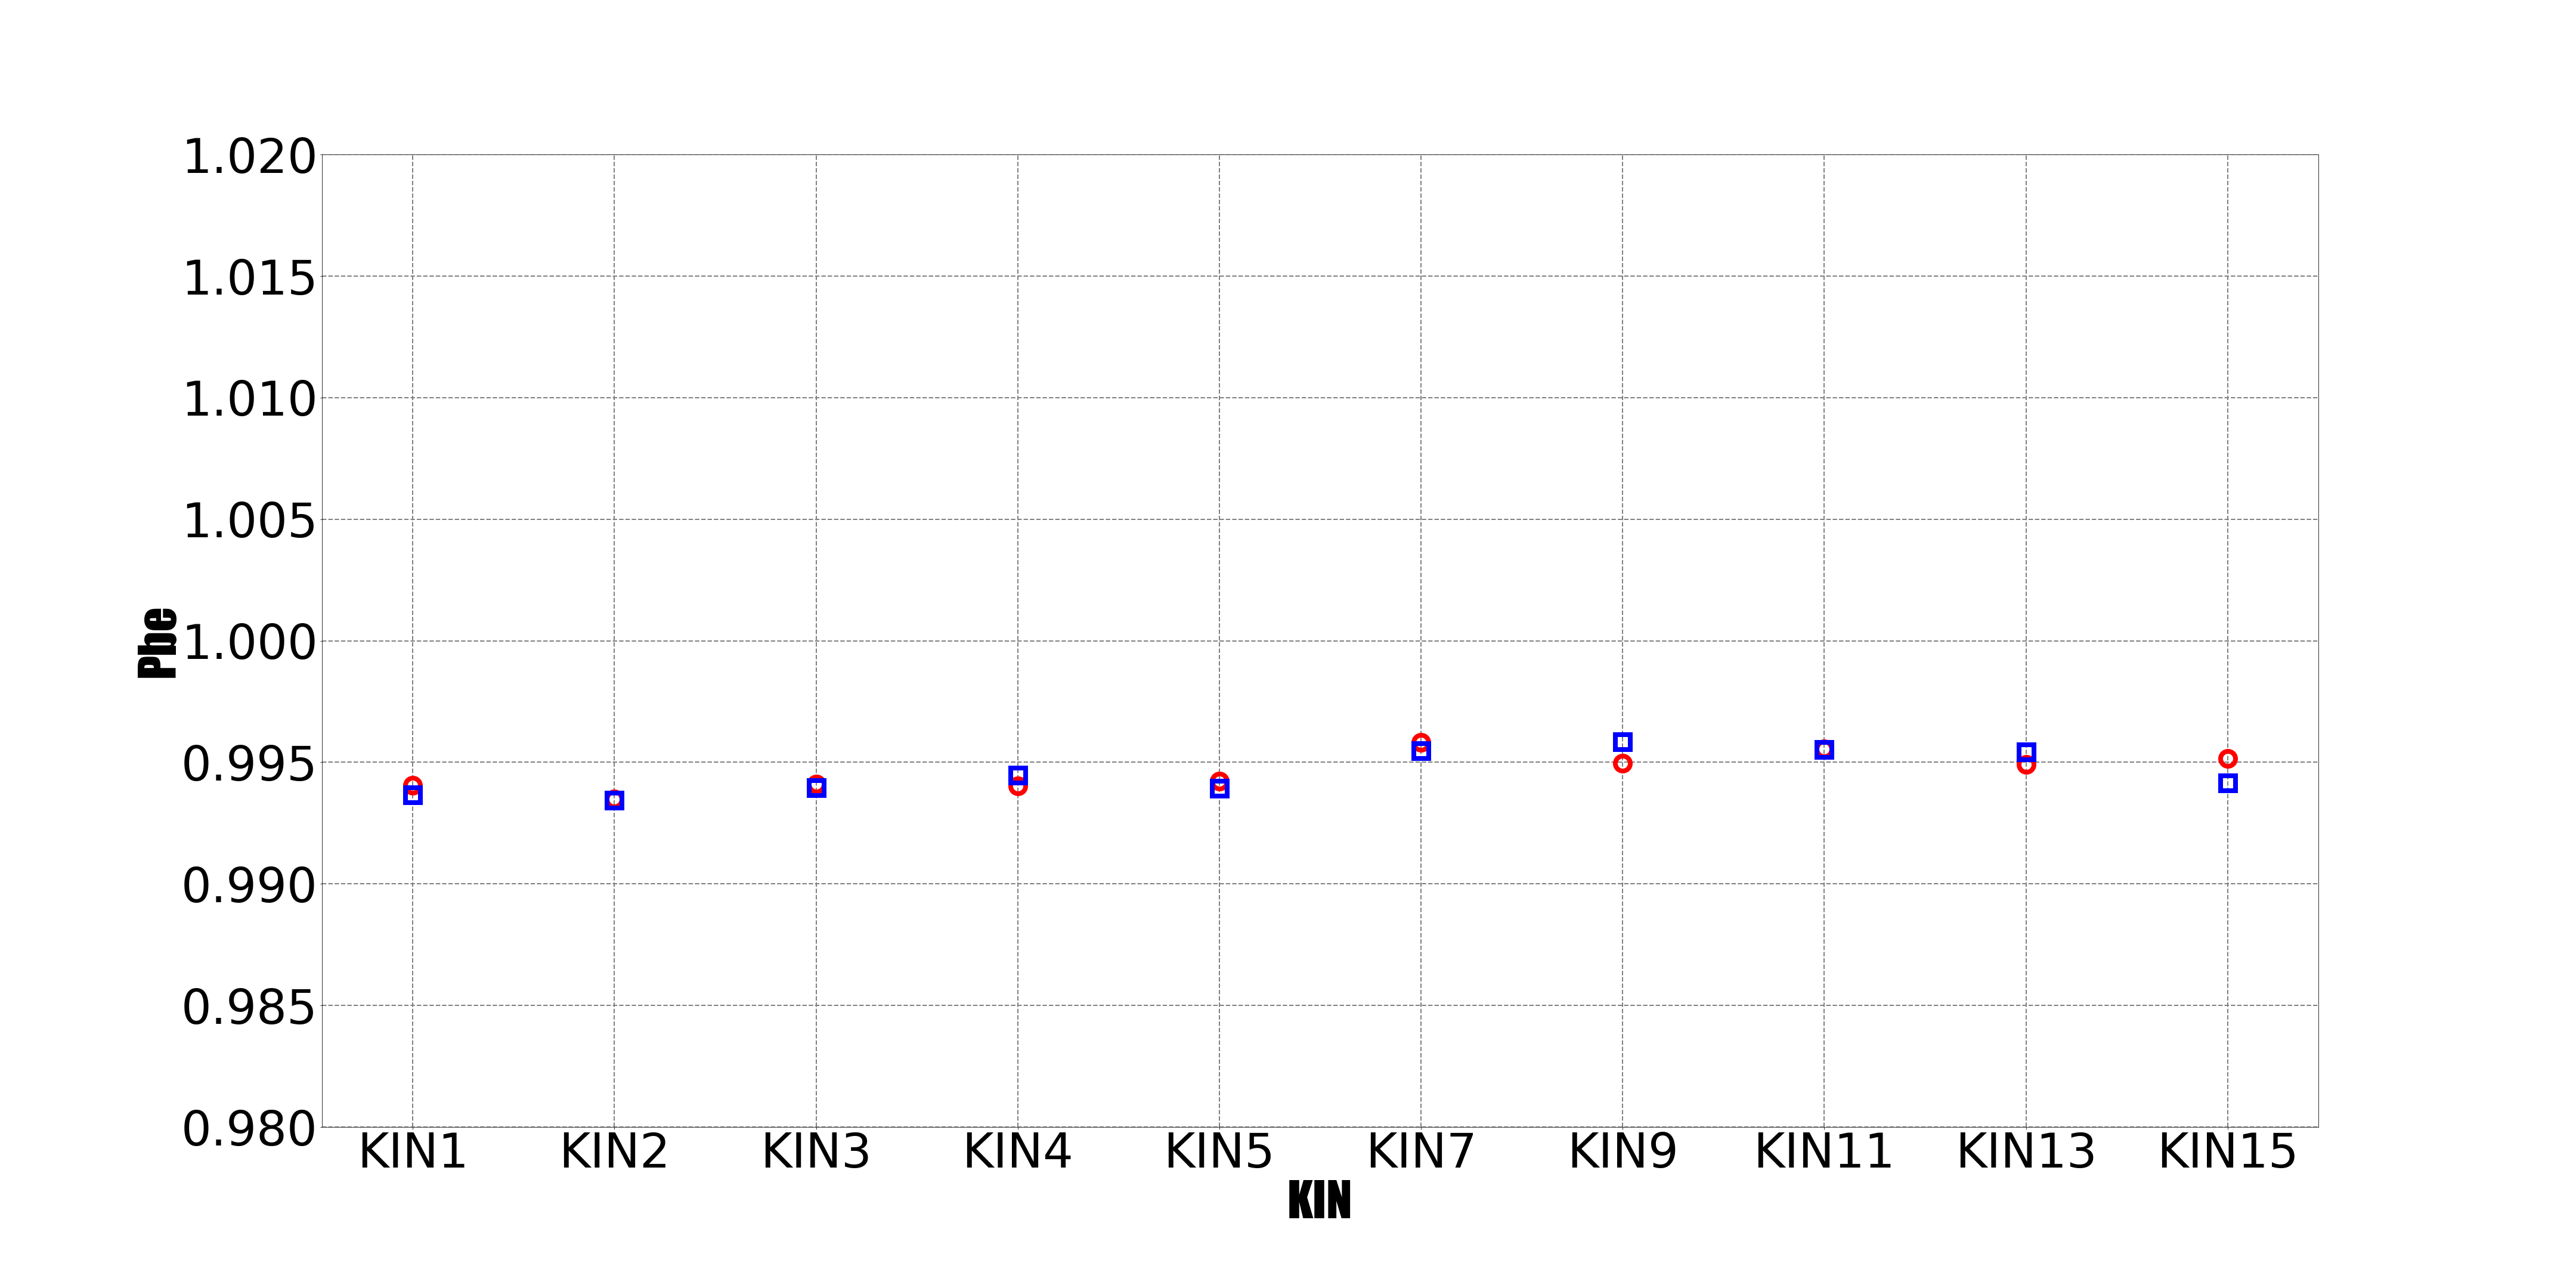
\includegraphics[width=3in]{./pid_plot/PIDD3.png}
\end{minipage}
}
\subfigure[electron effciency for calorimeter]{
\begin{minipage}[t]{1\linewidth}

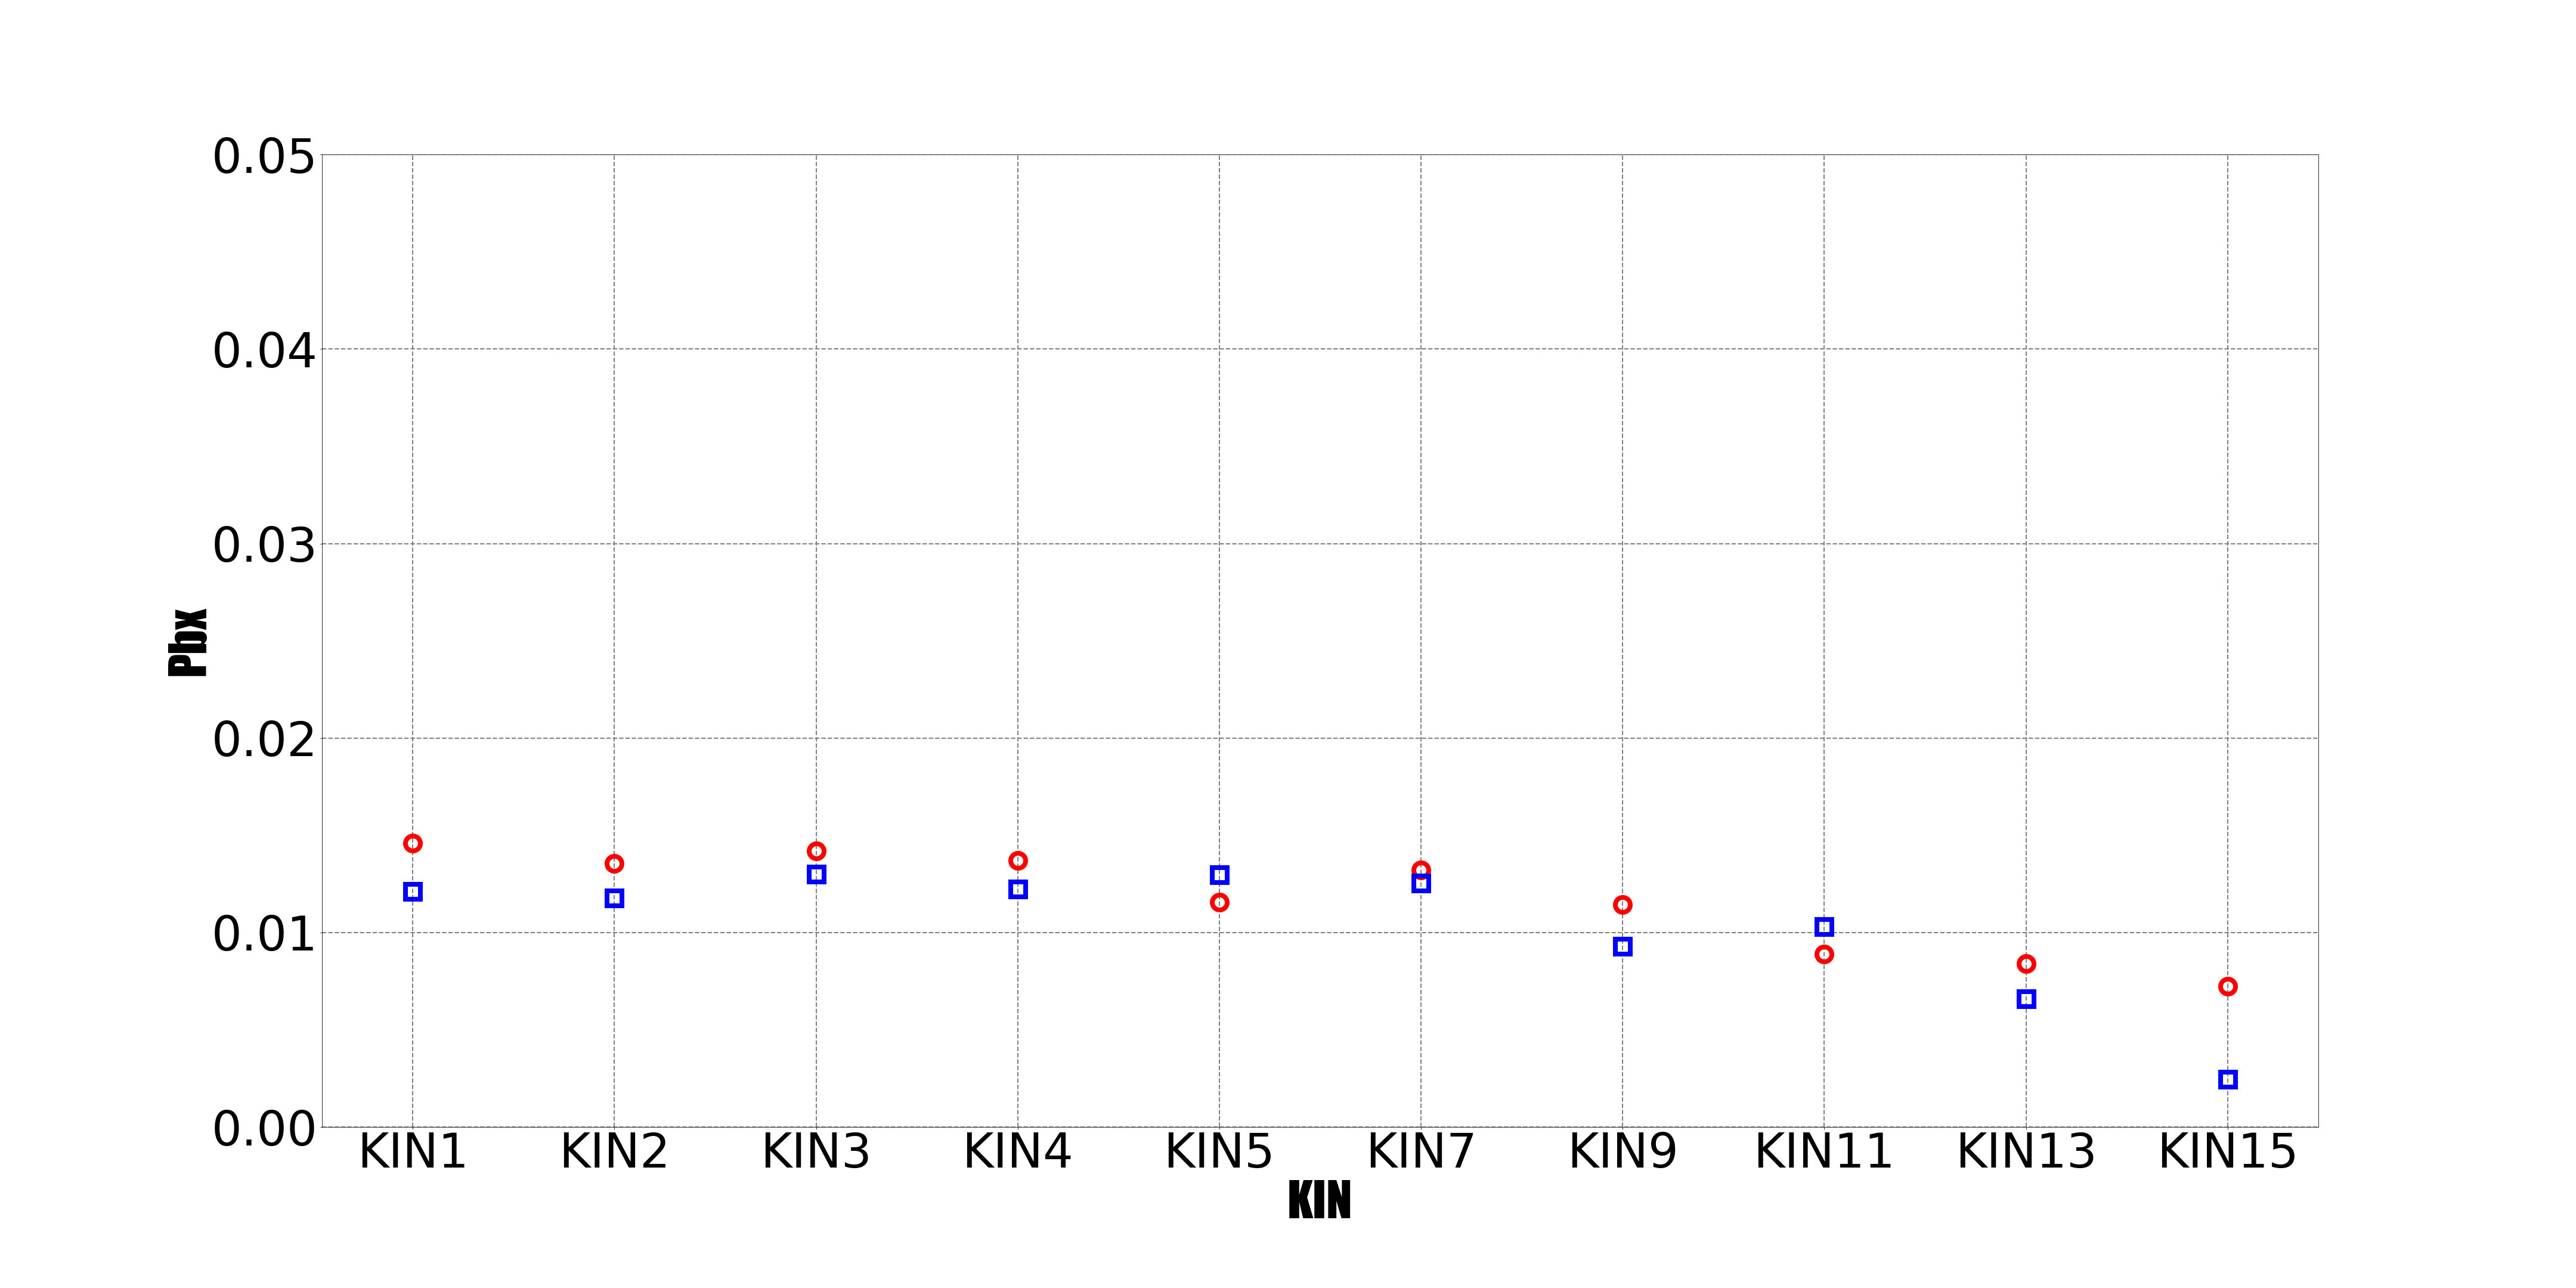
\includegraphics[width=3in]{./pid_plot/PID4.png}
\end{minipage}
}

\caption{The two PID efficiency for calorimeter with different kinematic settings  (Blue: He3 and Red: H3)  } \label{PPID4}
\end{figure}



 Since we only analysis electrons, for a certain PID cuts, we cares more about the non-electron contamination. Define 
\begin{equation}  
\left\{   \begin{array}{lr} 
             N_{e}^{TRUE}= P_{a}^{e} P_{b}^{e} N_{e}\\
             N_{e}^{FALSE}= P_{a}^{x} P_{b}^{x} N_{x}
             \end{array}  
\right.  
\end{equation}  
Where the $N_{e}^{FALSE}$ is the non-electron can pass our two PID cuts and $N_{e}^{TRUE}$ is the number of electrons can pass the same cuts, then the non-electron contamination can be calculated by the following 
\begin{equation}\label{eq:eff1}
\dfrac{x}{e}=\dfrac{N_{e}^{FALSE}}{N_{e}^{TRUE}+N_{e}^{FALSE}}
\end{equation}
Fig \ref{PPID5} shows the non-electron contamination at different kinematics settings, as we can see, this contamination is at 10-3 to 10-4 level (even smaller if only cross-section ratio be focused).                                                               
 
\begin{figure}
 	
 		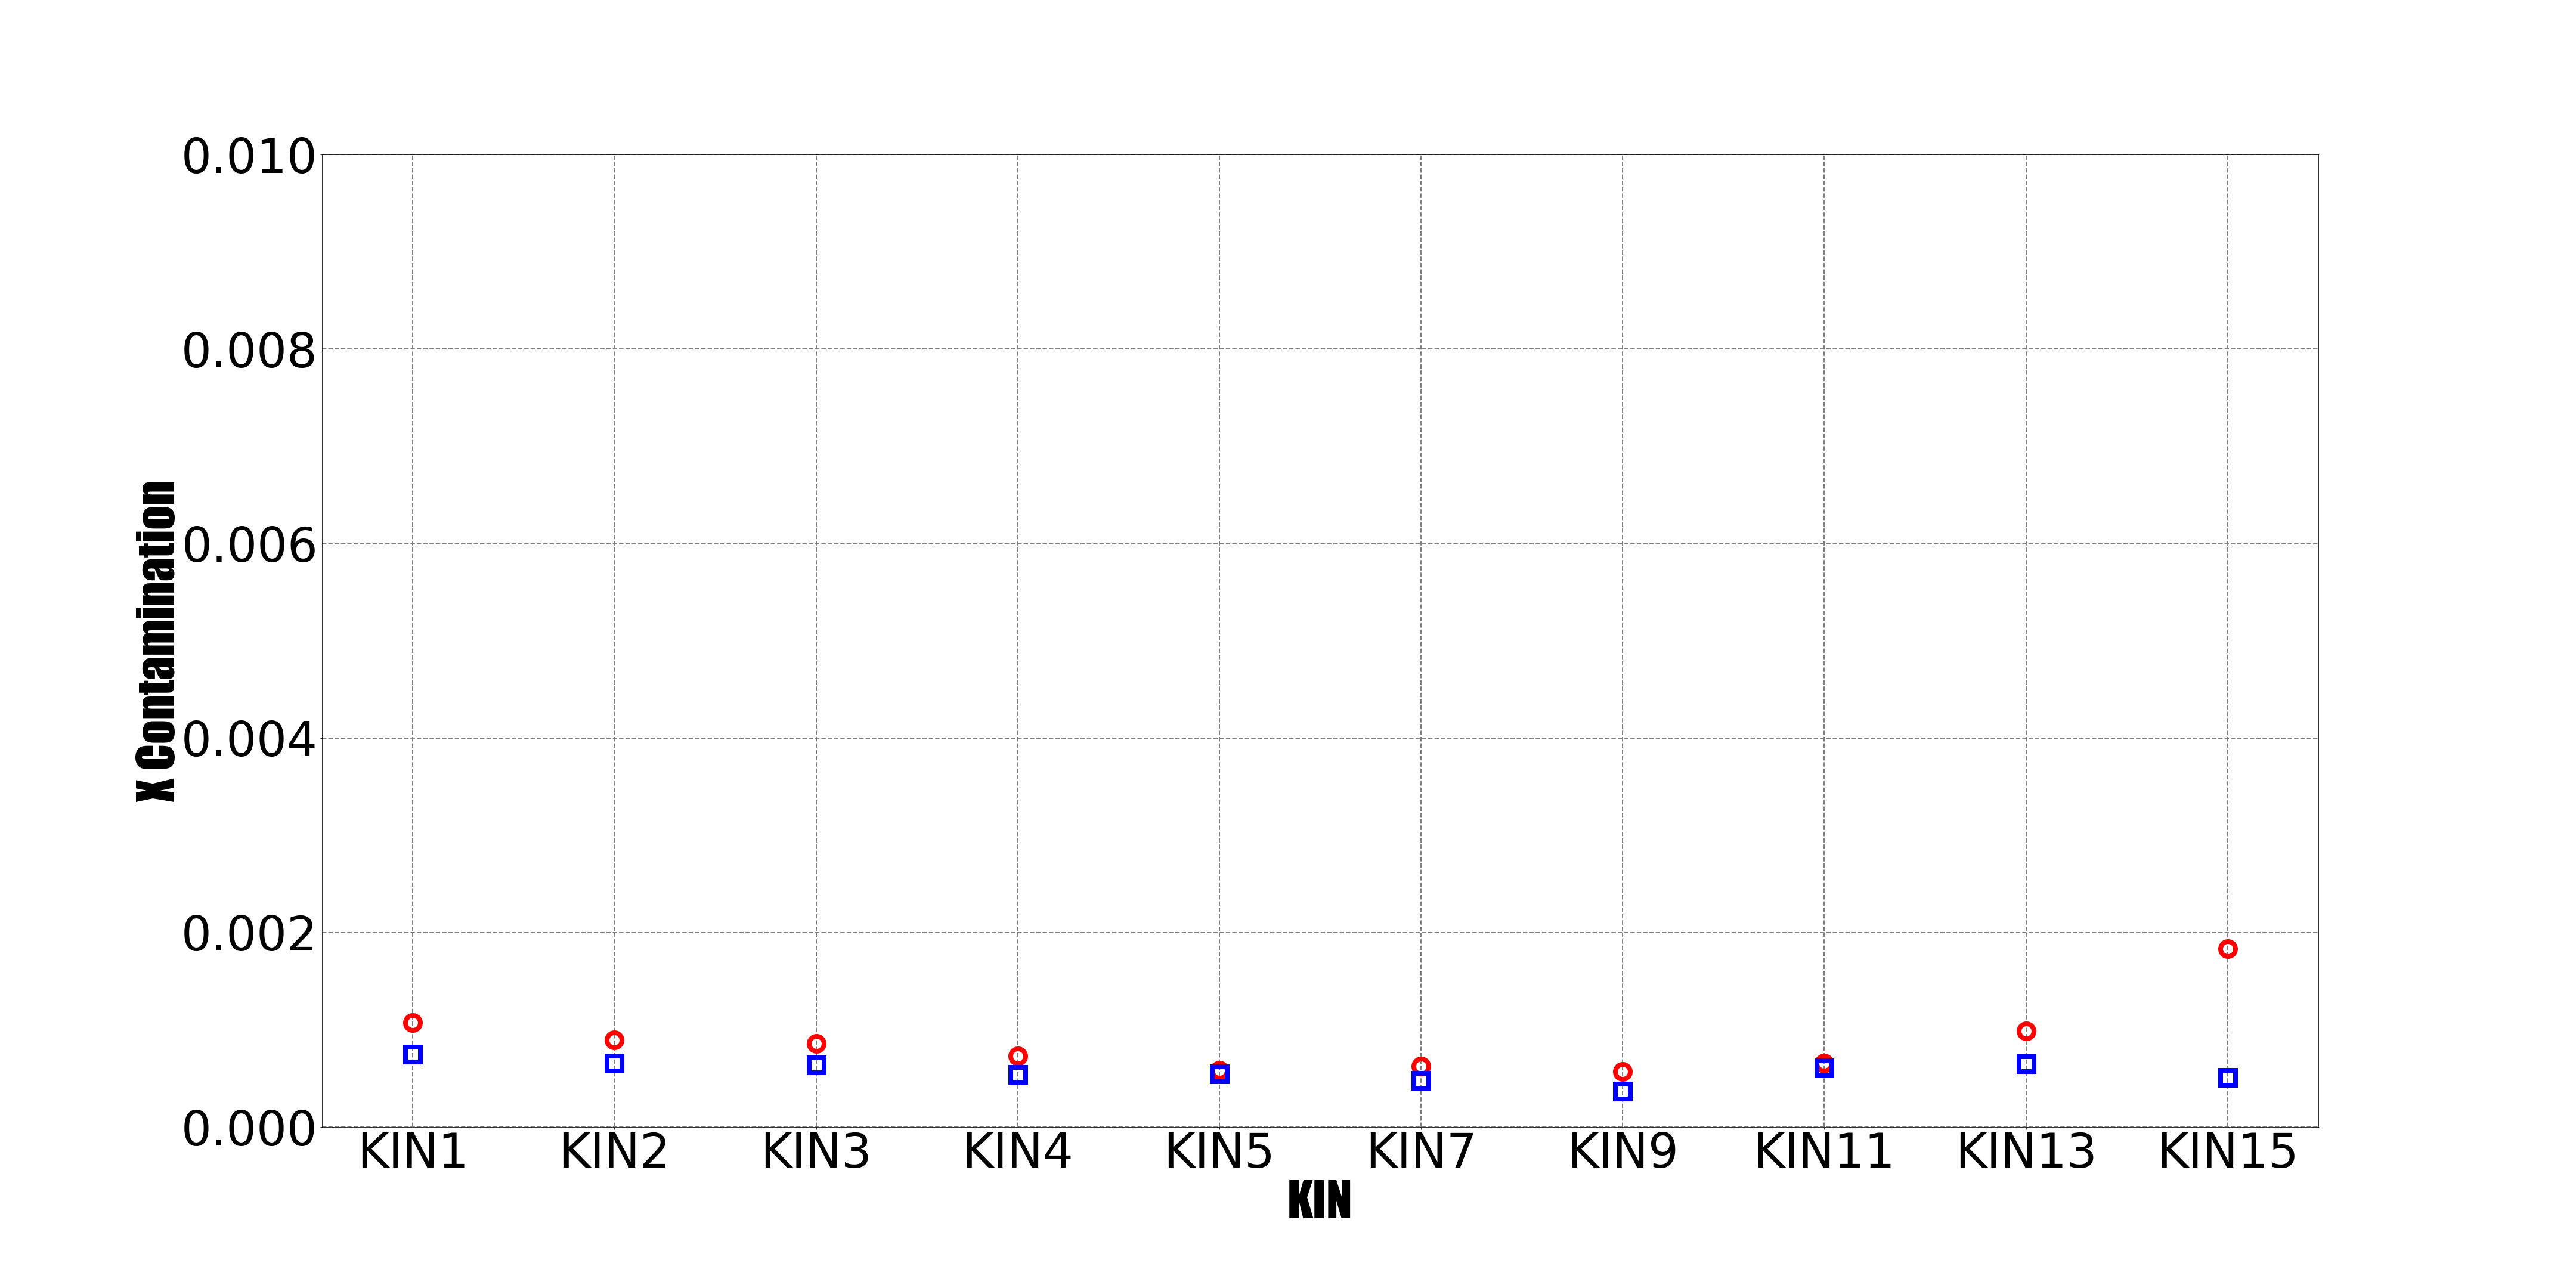
\includegraphics[width=0.5\textwidth]{./pid_plot/PID5.png}
 		\caption{ Non-electron contimination for H3(Red) and He3(Blue) with different kinematic setting  } \label{PPID5}
 	
\end{figure}   
 
%\bibliographystyle{plain}
%\bibliography{ref}




 \subsection{i. Positron Subtraction}
 (Tong Su)

 \subsection{ii. Endcap Subtraction}
 (Tong Su)

 \subsection{iii. Livetime}

 \subsection{iv. Tritium Decay}
 \subsection{Target composition}

Tritium decays to helium via the $\beta$-decay process $^3\text{H} \,\rightarrow\, ^3\text{He} + e^- + \overline{\nu}_e$, with a half-life of

\begin{equation*}
\tau_{1/2} = \ln(2)\tau = (4500 \pm 8) \text{ days} 
\end{equation*}

This results in a time-dependent target composition, with a decreasing (increasing) population of tritium (helium) nuclei.  These effects must be quantified and corrected in order to accurately extract the normalized tritium yield from tritium target data.

The target cell was filled with an initial tritium number density $n_T^0$, and initial helium number density $n_H^0$.  As tritium decays to helium, these number densities evolve in time as
\begin{align}
n_T &= n_T^0 \: e^{-t/\tau} \label{nT}\\[5pt]
n_H &= n_H^0(1 - e^{-t/\tau}) \label{nH},
\end{align}
where $t$ is the number of days since the target was filled.  Since the decay process preserves the total number of nuclei, the total number density $n_{tot}$ is constant in time:
\begin{align}
n_{tot} 	&= n_T + n_H \nonumber \\
		&= n_T^0 + n_H^0 
\end{align} 

With these quantities, the helium fraction can be defined:
\begin{equation}
f_H = \frac{n_H}{n_T + n_H} = \frac{n_H}{n_{tot}} \label{fH}
\end{equation}
Given an infinite amount of time, all of the tritium will decay to helium.  Therefore $f_H\rightarrow1$ as $t\rightarrow\infty$.  

\subsection{Normalized yield correction}

The normalized yield is defined as:
\begin{equation}
Y = \frac{N}{Qn},
\end{equation}
where $N$ is the number of detected electrons, $Q$ is the beam charge incident on the target, and $n$ is the target number density.  Assume that $N$ includes all corrections (deadtime, efficiency, endcap contamination, etc.) \textit{not} related to tritium decay.  In practice, the yield is extracted from multiple runs, so the number of detected electrons and luminosity must be summed over run number $i$:
\begin{equation}
Y = \frac{\sum N_i}{\sum Q_i n_i},
\end{equation}

The required correction must account not only for the evolution of the target composition (quantified in the previous section), but also for the fact that some of the detected electrons $N$ will have actually scattered from a helium nucleus instead of a tritium nucleus.  Begin by expressing the raw, uncorrected normalized yield (which is measured) as

\begin{equation}
Y_{raw} = \frac{\sum (T_i + H_i)}{\sum Q_i (n_{T,i} + n_{H,i})} \label{Yraw}
\end{equation}
where $T$ and $H$ are the number of detected electrons scattered by tritium and helium, respectively.  For time-dependent quantities (such as $n_{T,i}$ and $n_{H,i}$, given by Equations \ref{nT} and \ref{nH}), the subscript indicates the value of the quantity at the time of run $i$.  The goal is to obtain the normalized tritium yield $Y_T$ in terms of $Y_{raw}$ and correction factors, where

\begin{equation}
Y_T = \frac{\sum T_i}{\sum Q_i n_{T,i}}. 
\end{equation} 

Due to the helium contamination, the correction factor will depend on the normalized helium yield

\begin{equation}
Y_H = \frac{\sum H_i}{\sum Q_i n_{H,i}}. 
\end{equation}

From equation (\ref{Yraw}), only a few steps of algebra are required to obtain $Y_T$.  Recall that the total number density $n_{tot}=n_T + n_H$ is constant in time, and note that the tritium fraction $n_{T,i}/n = 1 - f_{H,i}$, where $f_H$ is the helium fraction defined by Equation \ref{fH}.

\begin{align*}
Y_{raw} 	&= \frac{\sum (T_i + H_i)}{\sum Q_i (n_{T,i} + n_{H,i})} \\[15pt]
		&= \frac{\sum T_i}{n_{tot} \sum Q_i} + \frac{\sum H_i}{n_{tot} \sum Q_i} \\[15pt]
		&= \left(\frac{\sum_i T_i}{\sum_i Q_i n_{T,i}}\right)\left(\frac{\sum_i Q_i n_{T,i}}{n_{tot} \sum_i Q_i}\right)
		+ \left(\frac{\sum_i H_i}{\sum_i Q_i n_{H,i}}\right)\left(\frac{\sum_i Q_i n_{H,i}}{n_{tot} \sum_i Q_i}\right) \\[15pt]
		&= Y_T\left(\frac{\sum Q_i(1-f_{H,i})}{\sum Q_i}\right) + Y_H\left(\frac{\sum Q_i f_{H,i}}{\sum Q_i}\right)
\end{align*}

To simplify notation, define the charge-averaged helium fraction:

\begin{equation}
\langle f_H \rangle \equiv \frac{\sum Q_i f_{H,i}}{\sum Q_i}
\end{equation}

Thus,

\begin{equation}
Y_{raw} = Y_T(1-\langle f_H \rangle) + Y_H \langle f_H \rangle,
\end{equation}

and finally,

\begin{equation}
Y_T = Y_{raw}\left(\frac{1}{1-\langle f_H \rangle}\right) - Y_H \left(\frac{\langle f_H \rangle}{1-\langle f_H \rangle}\right)
\end{equation}

\subsection{Uncertainty propagation}

Pending



 \subsection{v. Boiling}
 (Tong, Mike)

 \subsection{vi. Radiative Corrections}
 (Hanjie Liu)

\section{V. Binning and Combining}

 \subsection{Bin width Choice}

 \subsection{Bin Centering}

 \subsection{Combining Kinematic Overlap}

\end{document}

